\documentclass[10pt]{article}

\input{../preambule}
\input{../styles}
\input{../bas_de_page_quatrieme} 

%%%%%%%%%%%   Marges de pages  %%%%%%%%%%%%%%%% 
 \usepackage{geometry}
 \geometry{top=2cm, bottom=1cm, left=2cm , right=2cm}
%%%%%%%%%%%%%%%%%%%%%%%%%%%%%%%%%%%%%%%%%%%%%%%

%%%%%%%%%%%%%%%  Indentation  %%%%%%%%%%%%%%%%%%
\parindent=0pt
%%%%%%%%%%%%%%%%%%%%%%%%%%%%%%%%%%%%%%%%%%%%%%%%


\begin{document}

%%%%%%%%%%%%%%%%%%%%%%%%%%%%%%%%%%%%%%%%%%%%%%%
%%%%		 Titre encadré
%%%%%%%%%%%%%%%%%%%%%%%%%%%%%%%%%%%%%%%%%%%%%%%
\begin{encadrementombre}{Thème 10 Statistiques}
{\LARGE Statistiques}\\

%% Laisse la ligne vide ci-dessus
{\Large Gestion de donnée}
\end{encadrementombre}


%%%%%%%%%%%%%%%%%%%%%%%%%%%%%%%%%%%%%%%%%%%%%%%
%%%%		 Corps du document
%%%%%%%%%%%%%%%%%%%%%%%%%%%%%%%%%%%%%%%%%%%%%%%

%%%%%%%%%%%%%%%%%%%%%%%%%%%%%%%%%%%%%%%%%%%%%%%
%%%% \renewcommand{\arraystretch}{1.8}
\definecolor{shadecolor}{gray}{0.9}
%%%%%%%%%%%%%%%%%%%%%%%%%%%%%%%%%%%%%%%%%%%%%%%
%%%%%%%%%%%   Hauteur de ligne  %%%%%%%%%%%%%%%%
{\setlength{\baselineskip}{1.5\baselineskip}
%%%%%%%%%%%%%%%%%%%%%%%%%%%%%%%%%%%%%%%%%%%%%%%%


%%%%%%%%%%%%%%%%%%%%%%%%%%%%%%%%%%%%%%%%%%%%%%%%%%%%%%%
%     Notions
%%%%%%%%%%%%%%%%%%%%%%%%%%%%%%%%%%%%%%%%%%%%%%%%%%%%%%%
\section{Activités d'introduction}
\subsection{Effectifs et fréquences ( rappels)}
Voici les notes obtenues à un contrôle sur 10 par une classe de quatrième :\\
0 -- 1 -- 1 -- 2 -- 2 -- 2 -- 2 -- 3 -- 3 -- 4 -- 5 -- 5 -- 7 -- 7 -- 7--
8 -- 8 -- 10 -- 10 -- 10.

Compléter le tableau ci-dessous (voir éventuellement l'aide juste après) :\\
\strut\hskip 0pt plus 500pt minus 500pt%
\begin{tabular}{|p{4.2cm}*{11}{|p{5mm}}|}
\hline
Note
&
0 & 1 & 2& 3 & 4 & 5 & 6&7 &8 &9 &10 \\
\hline\hline
Effectifs
&
1 & 2 & 4&2 &&&& & && \\
\hline
Effectifs cumulés
&
1 & 3 & 7& 9&  & & & &
	 & & \\
\hline
Fréquences (en\%)
&
5\% & 10\% & 20\% & 10\% &  & & & & & & \\
\hline
Fréquences cumulées (en\%)
&
5\% & 15\% & 35\% & 45\% &  & & & & & & \\
\hline
\end{tabular}\hskip 0pt plus 500 pt minus 500 pt

\textbf{Effectifs -- Effectifs cumulés}\\%
	{Pour chaque note, {\em l'effectif} est le nombre d'élèves ayant
	eu cette note.\\
	Par exemple (dans le tableau), 1 élève a eu 0 ;
	2 élèves ont eu 1\dots\\ 
	Pour chaque note, {\em l'effectif cumulé} est le nombre d'élèves
	ayant eu cette note ou une note inférieure. Pour le calculer,
	il suffit à chaque fois de cumuler les effectifs.\\
	Par exemple (dans le tableau), 1 élève a eu 0 ;
	$1+2=3$ élèves ont eu 1 au plus ; $3+4=7$ élèves
	ont eu 2 au plus\dots}\\
\textbf{Fréquences -- Fréquences cumulées}\\%
	{Pour chaque note, {\em la fréquence} exprime la proportion d'élèves.\\
	Par exemple, sur les 20 élèves, 4 élèves ont eu une note de 2.
	La proportion est de 4 sur 20 ou $4\over20$ que l'on exprime
	en \%\ par le calcul $100\times{4\over20}=20$.\\
	Comme pour les effectifs cumulés, les {\em fréquences cumulées}
	sont obtenues en cumulant les fréquences.}

\subsection{Moyenne}
Voici les notes obtenues tout au long de l'année par un élève de 4\ieme\ en
mathématiques (toutes les notes sont sur 20) :\\
\begin{tabular}{|*{3}{p{3.5cm}|}}
\hline
\bf Trimestre 1 & \bf Trimestre 2 & \bf Trimestre 3 \\ \hline
12 -- 15 -- 7 -- 10 & 10 -- 12 -- 14 & 17 -- 11 -- 9 -- 14 -- 14 \\
\hline
\end{tabular}
\begin{enumerate}
\item Calculer la moyenne pour chaque trimestre. Calculer alors la moyenne
	annuelle. 
\item Calculer la moyenne de l'ensemble des notes obtenues tout au long
	de l'année. Quelle remarque peut-on faire ? Commenter.
	
\end{enumerate}

\newpage

\section{Cours}
\subsection{Moyenne d'une série statistique}
\begin{Df}
La \textbf{moyenne d’une série statistique} est le quotient de la somme
de TOUTES les valeurs par l’effectif total de cette série.
\end{Df}


\begin{Ex}
Voici les notes obtenues par Aurélie en Mathématiques au cours de l'année. 
\begin{itemize}
\item	1er trimestre :		10 – 9 – 11 – 12 – 11,5 – 14 – 12
\item	2ème trimestre :	9,5 – 11 – 12,5 – 8 – 13 – 18
\item	3ème trimestre :	8 – 9 – 14 – 12 – 10 – 13 – 11,5
\end{itemize}
Calculons sa moyenne annuelle :
		$m1 =\frac{10+9+11+\ldots{}+11,5}{20}=\frac{229}{20}=11,45$ 
\end{Ex}		
\begin{Rq}
La moyenne est toujours comprise entre la plus petite valeur
et la plus grande valeur de la série statistique.
\end{Rq}		
		
\subsubsection{Moyenne de moyennes}
Avec l'exemple précédent :
\begin{itemize}
\item 		1er trimestre :	  la moyenne d'Aurélie est $11,36$ ;
\item		2ème trimestre : la moyenne d'Aurélie est $12$ ;
\item		3ème trimestre : la moyenne d'Aurélie est $11,07$.
\end{itemize}
Calculons la moyenne de ses moyennes trimestrielles :
		$m2 =\frac{11,36+12+11,07}{3}=\frac{34,43}{3}$ donc  		$m2\approx 11,48$
		
\begin{Rq}	Cette moyenne est rarement égale à la moyenne de la série.
\end{Rq}

\subsection{Moyenne pondérée}

\begin{Df}
La \textbf{moyenne pondérée d’une série statistique} est le quotient de la somme
de TOUTES les valeurs multipliées chacune par leur coefficients
par la somme de ces coefficients.
\end{Df}


\begin{Ex}
\begin{multicols}{2}
Voici ci-contre la répartition par âge des membres d'un club d'échec.
Calculons l'âge moyen de ces membres.
	$a =\frac{5\times 13+6\times 14+7\times 15+5\times 16+6\times 17+3\times 18}{5+6+7+5+6+3}$\\  
	$a =\frac{490}{32}$\\ 
	$a = 15,3125$ \hspace{0.1cm}		soit environ 15 ans et 4 mois ($0,3125 \times 12 \approx 4$)\\

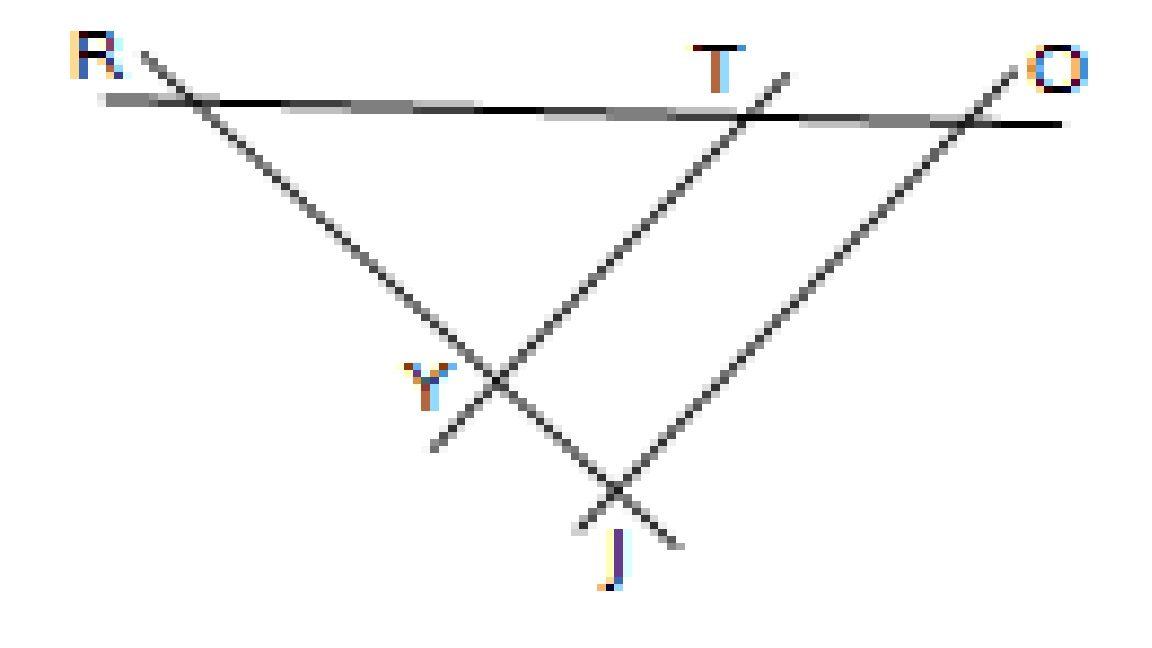
\includegraphics[scale=0.35]{cours1.jpg} 
\end{multicols}	
\end{Ex}
\section{Tableur}
\subsection{Moyenne}
\begin{shaded}
Lorsque l'effectif total d'une série statistique est \og  grand \fg{},
le tableur est un outil plus performant que la calculatrice pour calculer la moyenne.
\end{shaded}

\begin{Ex}
Sur la feuille de classeur ci-dessous,
on a calculé la longueur moyenne des prénoms des 684 élèves du collège.\\
		Les longueurs des prénoms sont rangées de la cellule C4 à la cellule C687.\\
		Ces cellules se suivent, on dit qu'elles sont contiguës.\\
		Dans la formule, on utilise alors le symbole \og  deux – points \fg{}.\\
		Dans la zone de saisie des fonctions, on a tapé : =MOYENNE(C4:C687).\\
		
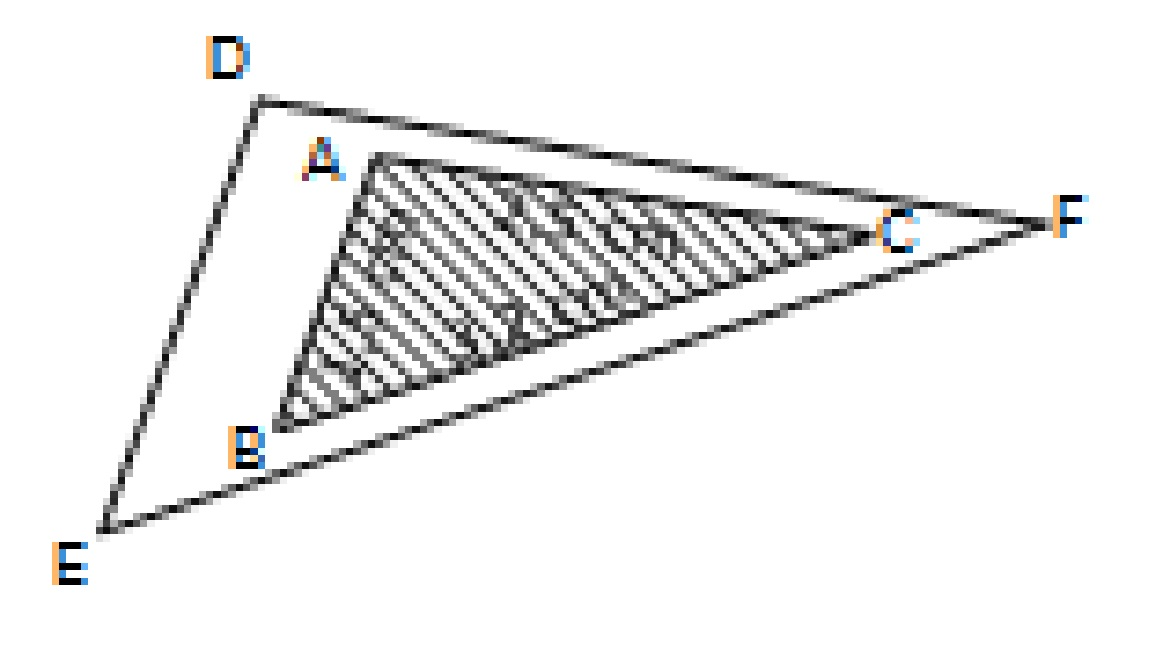
\includegraphics[scale=0.5]{cours2.jpg} 		
		
\end{Ex}


\begin{Ex} Calculons la moyenne des longueurs extrêmes.
		Le prénom le plus court, \og  Léa \fg{}, est dans la cellule B410.\\
		Le prénom le plus long, \og  Jean-Baptiste  \fg{}, est dans la cellule B624.\\
		Ces cellules ne se suivent pas, on dit qu'elles sont dis-contiguës.\\
		Dans la formule, on utilise alors le symbole \og  point – virgule \fg{}.\\
		Dans la zone de saisie des fonctions, on tape : =MOYENNE(B410;B624).
\end{Ex}
\newpage 

\subsection{Graphique}
\begin{shaded}
Le tableur permet également de créer rapidement des graphiques.
\end{shaded}

\begin{Ex}
A partir du fichier ci-dessus, on a créé la nouvelle feuille de calcul ci-dessous.
\begin{multicols}{2}
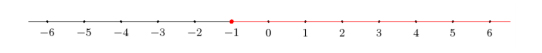
\includegraphics[scale=0.3]{cours3.jpg}
\vspace{0.5cm}\\
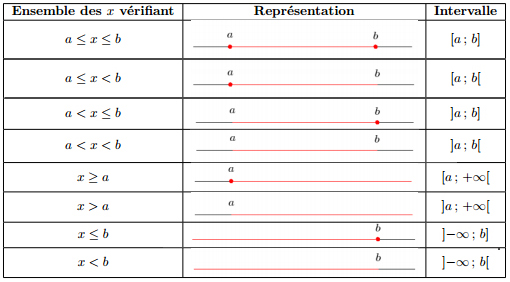
\includegraphics[scale=0.3]{cours4.jpg}  
\end{multicols}

Voici comment obtenir le graphique ci-dessus avec OpenOffice ou Excell.
Sélectionner la plage de cellules D2:E14. Dans le menu Insertion, choisir Diagramme… 
\begin{itemize}
\item Étape 1 : choisir XY(dispersion) et Points et lignes comme type de diagramme. Suivant >>
\item Étape 2 : choisir Série de données en colonnes et Première ligne comme étiquette. Suivant >>
\item Étape 3 : Suivant >>
\item Étape 4 : Titre : Répartition des prénoms – Sous-titre : en fonction de leur longueur.\\
		Axe X : Longueur des prénoms – Axe Y : Effectifs.\\ 
		Afficher les grilles : coche les deux cases Axe X et Axe Y.\\
		Décocher la case Afficher la légende.\\ Terminer >>\\
Cliquer en dehors de la zone du graphique pour revenir à la feuille de classeur.
\end{itemize}
\end{Ex}








\newpage

\section{Quelques Exercices}

\begin{Exo}
Voici les notes d'un élève de 4\ieme\ en mathématiques.
\medskip
\begin{enumerate}
 \item [1\ier\ trimestre] 15\kern5mm 10\kern5mm 8\kern5mm 13\kern5mm 10
\item[2\ieme\ trimestre] 13\kern5mm 9\kern5mm 7\kern5mm 14\kern5mm 13\kern5mm 16
\item[3\ieme\ trimestre] 12\kern5mm 15\kern5mm 17\kern5mm 14\kern5mm 12
\end{enumerate}
\begin{enumerate}
  \item Calcule sa moyenne pour chacun des trois trimestres.
  \item Calcule la moyenne des moyennes des trois trimestres.
  \item Calcule la moyenne de l'ensemble de ses notes sur son année de 4\ieme.\\Que remarque-t-on ?
\end{enumerate}

%@Commentaire: Travail intéressant sur la définition d'une moyenne sur un bulletin.
\end{Exo}

\begin{Exo}
Pierre, Jean et Alain ont passé un examen comportant quatre
disciplines. Pour être reçu, il faut atteindre 10 de moyenne.
\begin{enumerate}
\item Calcule la moyenne, sans coefficient, des trois candidats.
\begin{center}
  \begin{tabular}{|c|c|c|c|c|}
\cline{2-5}
\multicolumn{1}{c|}{}&Français&Mathématiques&Anglais&Technologie\\
\hline
Pierre&15&9&11&7\\
\hline
Jean&10&11&12&9\\
\hline
Alain&7&14&13&8\\
\hline
  \end{tabular}
\end{center}
\item Pour cet examen, le français, les mathématiques, l'anglais et la
technologie ont respectivement pour coefficient 6; 4; 2 et 5.\par
Calcule la moyenne pondérée de chaque candidat et dis s'ils sont reçus
ou non.
\end{enumerate}
%@Commentaire: Exercice concret pour les élèves.
\end{Exo}



\begin{Exo}
Voici les notes obtenues à un contrôle sur 10 par une classe de quatrième :\\
0 -- 1 -- 1 -- 2 -- 2 -- 2 -- 2 -- 3 -- 3 -- 4 -- 5 -- 5 -- 7 -- 7 -- 7--
8 -- 8 -- 10 -- 10 -- 10.
\begin{enumerate}
\item Calculer la moyenne de la classe pour ce contrôle.
\item Pour accélérer les calculs, par quelle opération aurait-on pu
	remplacer certaines séries de notes identiques ?
\end{enumerate}
\end{Exo}

\begin{Exo}
Lors d'un test d'endurance, plusieurs élèves ont eu 12 minutes pour
parcourir la plus grande distance possible. Voici les résultats des
élèves :
2230 -- 2450 -- 1890 -- 1850 -- 2650 -- 2630 -- 2110 -- 2250 -- 2180 --
1980 -- 2000 -- 2850 -- 1950 -- 2920 -- 1975 -- 1910 -- 1860 -- 1930 --
2010 -- 2400 -- 2650 -- 2320 -- 2190 -- 2730 -- 2120 -- 2380 -- 2220.

\begin{enumerate}
\item
On veut calculer la moyenne approximative des distances parcourues.
Pour cela, dénombrer le nombre d'élèves dans chacun des intervalles
suivants :\\
\hskip 0pt plus 500pt minus 500pt\begin{tabular}{|*{6}{c|}}
\hline
$[1800 ; 2000 [$ & $[2000 ; 2200 [$ &
$[2200 ; 2400 [$ & $[2400 ; 2600 [$ &
$[2600 ; 2800 [$ & $[2800 ; 3000 [$ \\
\hline
&&
 &&& \\
\hline
\end{tabular}\hskip 0pt plus 500 pt minus 500 pt\strut
\item
Calculer une moyenne approchée en remplaçant la distance de chaque élève
	par le début de chaque intervalle (1800 pour le premier, 2000 pour
	le deuxième,\dots) en pensant à remplacer chaque série de nombres
	identiques par une multiplication.
	
\item Reprendre la question précédente en 
	remplaçant la distance de chaque élève
	par le milieu de chaque intervalle (1900 pour le premier, 2100 pour
	le deuxième,\dots)
	
\item Reprendre la question précédente en 
	remplaçant la distance de chaque élève
	par la fin de chaque intervalle (2000 pour le premier, 2200 pour
	le deuxième,\dots)
	
\item La moyenne exacte est d'environ 2246.\\
Quelle était la meilleur moyenne approchée. Commenter.%60635/27
\end{enumerate}
\end{Exo}

\begin{Exo}
Le professeur d'EPS a relevé les performances ci-dessous :
\begin{center}
  \begin{tabularx}{0.85\linewidth}{|l|X|X|l|X|X|}
    \hline
\multicolumn{1}{|c|}{Noms}&Temps au 80~m (s)&Hauteur du saut (cm)&\multicolumn{1}{c|}{Noms}&Temps au 80~m (s)&Hauteur du saut (cm)\\
\hline
Charles&\multicolumn{1}{c|}{13}&\multicolumn{1}{c|}{110}&Gérald&\multicolumn{1}{c|}{13,6}&\multicolumn{1}{c|}{115}\\
Bruno&\multicolumn{1}{c|}{12,5}&\multicolumn{1}{c|}{120}&Nicolas&\multicolumn{1}{c|}{13,9}&\multicolumn{1}{c|}{110}\\
Sylvie&\multicolumn{1}{c|}{15}&\multicolumn{1}{c|}{100}&Florence&\multicolumn{1}{c|}{14,7}&\multicolumn{1}{c|}{110}\\
Brice&\multicolumn{1}{c|}{13,2}&\multicolumn{1}{c|}{125}&Daniel&\multicolumn{1}{c|}{13}&\multicolumn{1}{c|}{125}\\
Carine&\multicolumn{1}{c|}{15,4}&\multicolumn{1}{c|}{100}&Viviane&\multicolumn{1}{c|}{16}&\multicolumn{1}{c|}{95}\\
Léon&\multicolumn{1}{c|}{12}&\multicolumn{1}{c|}{135}&Barbara&\multicolumn{1}{c|}{15,1}&\multicolumn{1}{c|}{105}\\
Christian&\multicolumn{1}{c|}{12,6}&\multicolumn{1}{c|}{130}&Jeanne&\multicolumn{1}{c|}{14,9}&\multicolumn{1}{c|}{110}\\
\'Elisabeth&\multicolumn{1}{c|}{15,4}&\multicolumn{1}{c|}{95}&Lucie&\multicolumn{1}{c|}{15,4}&\multicolumn{1}{c|}{100}\\
Aude&\multicolumn{1}{c|}{14,9}&\multicolumn{1}{c|}{110}&Odile&\multicolumn{1}{c|}{14,2}&\multicolumn{1}{c|}{85}\\
Cécile&\multicolumn{1}{c|}{16,2}&\multicolumn{1}{c|}{85}&Alice&\multicolumn{1}{c|}{15,6}&\multicolumn{1}{c|}{105}\\
Clément&\multicolumn{1}{c|}{12}&\multicolumn{1}{c|}{140}&Gaël&\multicolumn{1}{c|}{13,5}&\multicolumn{1}{c|}{125}\\
Cathy&\multicolumn{1}{c|}{15,8}&\multicolumn{1}{c|}{100}&Pierre&\multicolumn{1}{c|}{12,3}&\multicolumn{1}{c|}{135}\\
Delphine&\multicolumn{1}{c|}{15}&\multicolumn{1}{c|}{105}&Armand&\multicolumn{1}{c|}{12,8}&\multicolumn{1}{c|}{130}\\
Jacques&\multicolumn{1}{c|}{13,1}&\multicolumn{1}{c|}{135}&Jean&\multicolumn{1}{c|}{13,1}&\multicolumn{1}{c|}{115}\\
André&\multicolumn{1}{c|}{13,9}&\multicolumn{1}{c|}{120}&David&\multicolumn{1}{c|}{12,5}&\multicolumn{1}{c|}{135}\\
\hline
  \end{tabularx}
\end{center}
\begin{enumerate}
  \item
    \begin{enumerate}
    \item Quel est le temps moyen mis pour effectuer le 80~m ?
    \item Combien d'élèves ont un temps supérieur au temps moyen ?
    \end{enumerate}
  \item
    \begin{enumerate}
    \item Quelle est la hauteur moyenne d'un saut ?
    \item Combien d'élèves ont une hauteur inférieure à la hauteur
      moyenne ?
    \end{enumerate}
\end{enumerate}
\end{Exo}

\end{document}